\documentclass{standalone}
\usepackage{pgfplots}
\usepackage{pgfplotstable}
\pgfplotsset{width=9cm, compat=1.5}
\begin{document}
	\begin{tikzpicture}
	\begin{axis}[
	legend style={nodes={scale=0.6, transform shape},  font=\large, draw=none},
	legend pos= north west,
	xlabel=$\varepsilon$,
	ylabel=Magnetizaci\'on $(\mu_B/celda)$]
	
	\addplot table [x=e, y=mag] {magn.dat};
	\addlegendentry{Magnetizaci\'on};
	\addplot table [x=e, y={create col/linear regression={y=mag}}]{magn.dat};
	\addlegendentry{%
		$\pgfmathprintnumber{\pgfplotstableregressiona} \cdot x
		\pgfmathprintnumber[print sign]{\pgfplotstableregressionb}$ ajuste} %
	
	
	\node at (510,150) {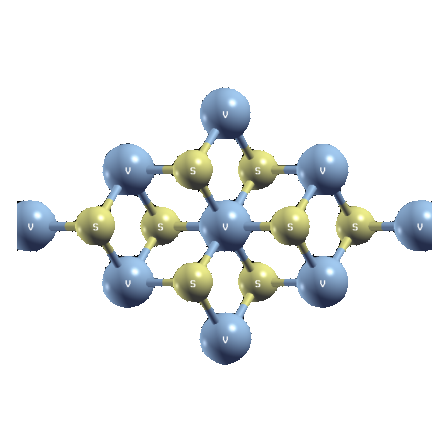
\includegraphics[scale=0.17]{est_0.0}};
	\node at (730,720) {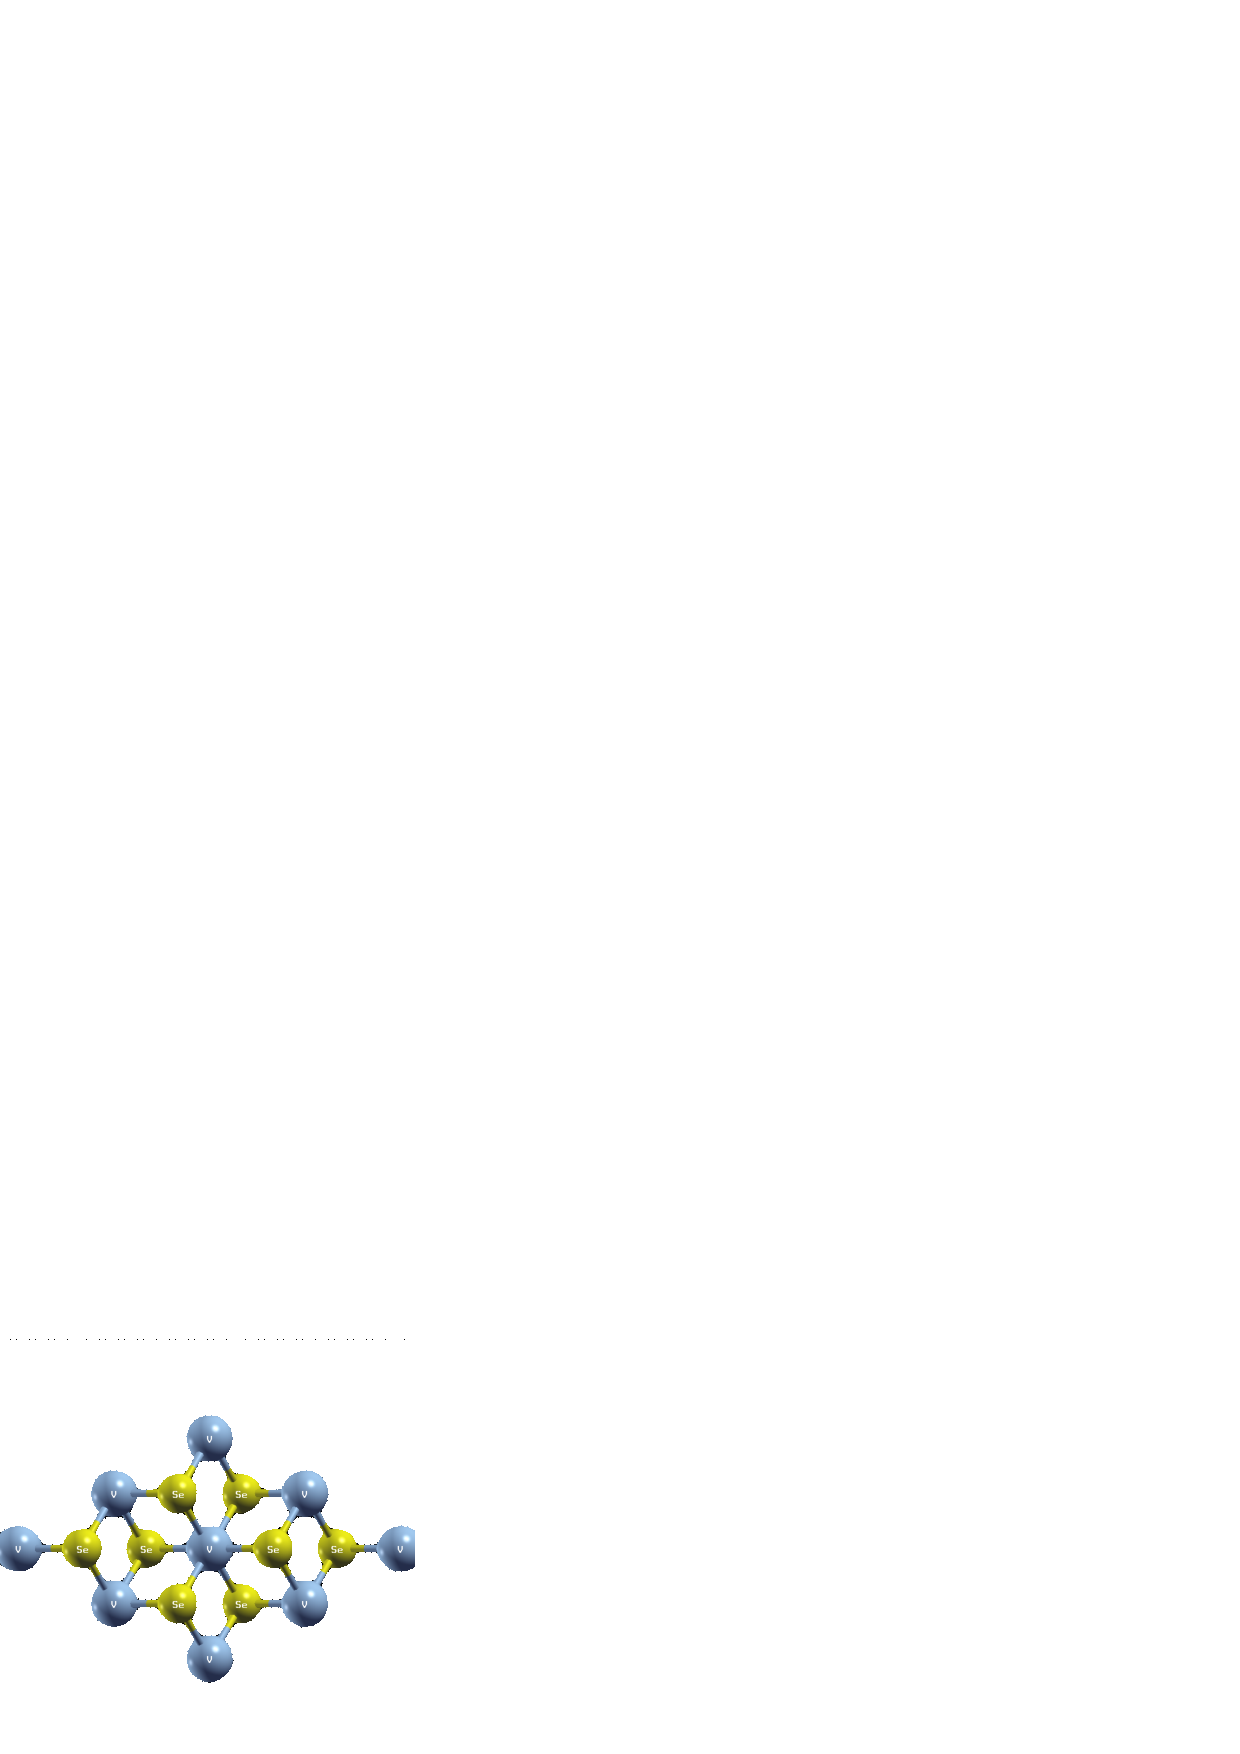
\includegraphics[scale=0.17]{est_0.05}};
	\node at (40,250) {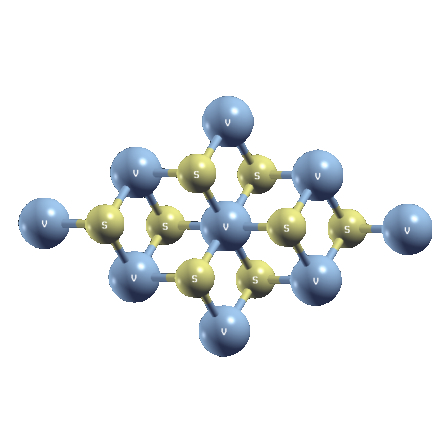
\includegraphics[scale=0.17]{est_-0.05}};
	\draw[->, color=black, very thick](50,130)--(10,10);
	\draw[->, color=black, very thick](840,710)--(980,770);
	\draw[->, color=black, very thick](490,240)--(500,300);
	\end{axis}
	
	\end{tikzpicture}
\end{document}
